\documentclass[../../dd.tex]{subfiles}

% Document
\begin{document}
\chapter{Development and testing}
    \section{Overview}
	The purpose of this chapter is to detail the approach and the techniques used during the development process of the application. Given the nature of the application, it is important to clarify the plan that guided all the phases of the software development in order to achieve the final result.

	\section{Development approach}
    The development of the application has been carried out following a \textbf{test-driven} approach. In particular the components have been developed in parallel to a series of
	\textbf{widget tests} written with the purpose of matching the developed components with the expected behaviour. The order of the components has been established considering
	a \textbf{bottom-up} development plan, which starts from simple and atomic components used to model more complex widgets and views. In particular basic widgets like buttons, boxes,
	forms and other frequently used components have been developed first and immediately \textbf{unit-tested}.

	\section{Testing}
	To implement the system, we decided to test the application mainly through debug on both emulators and real devices. The only exception is the \textbf{mobile application}, for which we also performed unit testing on the main UI components and subsequent integration testing to verify the compatibility among them. In particular separable widgets used by multiple components of the application have been tested using a particular type of test supported by Flutter, the widget tests. We then developed a special integration test suite using the Flutter driver to verify the correct behavior of the application as a whole.

	\subsection{Widget tests}
	Widget tests are simply \textbf{unit-tests} performed in an environment that allows to test the behaviour of a widget class. The goal of this approach is to verify that the tested  widget’s \textbf{UI} looks and interacts as expected. This operations involves multiple classes and requires a test environment able to support the entire widget lifecycle. In the specific context of the application, the tests carried out verified the behavior of the widget by injecting an input and verifying the presence of the expected elements through the finder. A \textbf{finder} is a class provided by the test environment used to locate widgets and elements inside the pumped widget. If the finder is able to locate the expected element with the expected features and properties the test is passed.\\

	\textbf{Case study: Rating stars}\\
	This example is provided with the purpose of clarifying the general structure of one of the developed widget tests. \\
	The tested widget is a bar used to visualize the average rate of the reviews left to a caregiver account. This is done by the mean of series of star icons representing the average value of the user profile. In this case we are verifying if the icons representing the stars are consistent with the numeric value of the average rate.  Below the code of the test.

    \vspace{2 mm}
    \lstinputlisting{assets/code/rating_stars_widget_test.dart}
    \vspace{8 mm}

	As it can be seen, the test has the purpose of verifying that the number and the type of the icons rendered by the widget is consistent with the decimal value representing the average rate of the caregiver. The test involves multiples scenarios that consider also the approximations carried out in presence of particular values.
	Following this approach we have developed a number of tests consistent with the separable components used to build the application. The other performed widget tests are those reported below.

	 \begin{figure}[H]
        \centering
        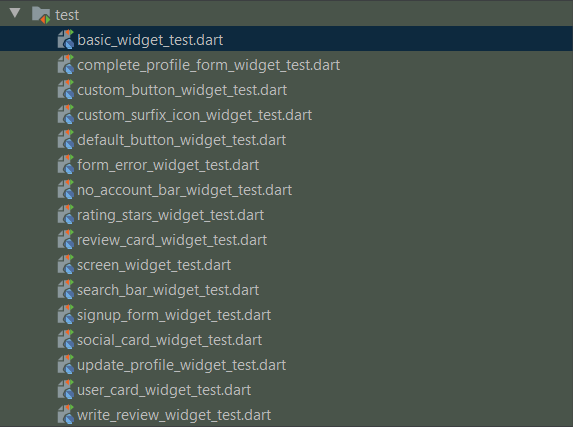
\includegraphics[scale=1.25]{../../assets/widget_tests.png}
        \caption{Performed widget tests}\label{fig:widget-tests}
    \end{figure}

    \subsection{Integration tests}
	Widget tests generally do not check how individual components interact with each other and do not capture the performance of an application running on a device. To evaluate the correct behavior of an application based on different interacting modules we have to rely on a specific test suite that guides the application by verifying that everything works correctly along the way. With these considerations in mind we developed a suite of integration tests using the package \textbf{flutter\_driver}. The basic approach is to deploy an instrumented application to a real device or emulator and then “drive” the application from a separate test suite. In our case the test suite performs the operations related to the registration of a caregiver user and then continue by using the app in order to test its main features. These process was implemented by using the core features of the driver package of Flutter. For every test, we first created the \textbf{SerializableFinders} to locate specific widgets, then we connected to the app before our tests run in the \textbf{setUpAll()} function. After that we have structured the workflow of the relevant scenarios by considering the main use cases of the application. Eventually, we disconnected from the app in the \textbf{teardownAll()} function after the tests were completed.\\
    The code snippets below show the implementation of the initialization phase and a couple of tests performed on different screens of the application.

	\vspace{2 mm}
    \lstinputlisting{assets/code/integration.dart}
    \vspace{8 mm}


\end{document}
